\section{Case Study}

The primary motivation for this work is to improve probabilistic forecasts of wind power production, following the framework of \citet{jorgensenSequentialMethodsError2025}. To ensure a direct comparison with their results, we use the same dataset and modeling conditions.

\subsection{Data}

The dataset consists of observed wind-power production and an ensemble of physically based production forecasts for the two Danish electricity bidding zones, DK1 and DK2, each further divided into onshore and offshore wind production.
The two zones differ substantially in geography, installed capacity, and interconnection structure:

\begin{itemize}
    \item DK1 is interconnected with continental Europe.
    \item DK2 is interconnected with the Nordic countries.
\end{itemize}

Each zone exhibits distinct production dynamics, but the time series show clear cross-zone correlation.
Notably, DK1 onshore has by far the largest installed capacity—approximately equal to the other three subzones combined.

A representative example of the full dataset is shown in \cref{caseproduction}.

\begin{figure}[htb]
    \centering
    \includegraphics[width=\linewidth]{Results/Graphs/data_example.pdf}
    \caption{Caption}
    \label{casedata}
\end{figure}

\subsubsection{Observed power Production}
\label{case-data-observed}
Observed production data spans the period
2022‑01‑01 00:00:00 to 2024‑10‑12 23:00:00,
obtained from the Danish TSO Energinet, via their open data service
\href{https://www.energidataservice.dk/}{Energi Data Service} \citep{energinetEnergiDataService}.

The data used here is from the dataset for statistical use. This means that data is only available after a considerable wait (days to weeks). As an alternative Energinet also provides a real-time dataset.

A statistical summary of the observed production for all four zones is provided in \cref{tab:data:observation}.

\begin{table}[htb]
\begin{tabular}{lrrrr}
\toprule
 & DK1-offshore & DK1-onshore & DK2-offshore & DK2-onshore \\
\midrule
mean & 599.49 & 1058.72 & 425.28 & 197.99 \\
std & 408.40 & 876.60 & 330.13 & 173.08 \\
min & 0.01 & 0.83 & 0.01 & 0.01 \\
25% & 209.92 & 317.97 & 105.30 & 48.56 \\
50% & 590.10 & 836.06 & 369.83 & 147.35 \\
75% & 976.31 & 1606.89 & 754.12 & 319.61 \\
max & 1364.77 & 3556.59 & 983.61 & 684.24 \\
\bottomrule
\end{tabular}
\end{table}


\subsubsection{Ensemble forecast}
The dataset also includes ensemble forecasts derived from ECMWF weather forecasts. Forecasts are provided at hourly resolution, and each day’s forecast is issued 12 hours before the target day.

\begin{itemize}
    \item 1 high‑probability ensemble (HPE)
    \item 50 perturbed ensemble members, generated by perturbing the initial conditions of the HPE.
\end{itemize}

Thus, each forecast consists of 51 physically simulated scenarios for each zone.

The weather forecast from the ECMWF is directly converted into of forecasted power production by a proprietary methods. 

Due to the proprietery nature of the neither the provider of, nor the full data can be disclosed 

Some anomalies are present particularly for DK2‑onshore, where forecasts occasionally collapse to a constant value of approximately 315 kWh. This is a known artefact of the generating process and is undesirable.

Another systematic effect arises from curtailment. At certain times, producers are paid to reduce generation due to market or transmission constraints, leading to artificially low production values. Prior work removed such periods, as they are not representative of unconstrained physical generation. In contrast, we retain these periods, as they reflect real‑world operational conditions.

\subsection{Data Cleaning}

Only light preprocessing of data was necessary:

\begin{itemize}
    \item Zero‑valued observations: Observations equal to exactly zero lead to numerical instability during the probability‑integral-transform stage of the pipeline. To avoid this, values of 0 were replaced with a small positive constant (0.01), which is practically indistinguishable at operational scales.
    \item Timestamp harmonization: he observational and ensemble datasets used slightly different timestamp formats. Both were converted to UTC to ensure alignment
\end{itemize} 

No additional filtering or smoothing was applied.

\subsection{Data Split}

We adopt a straightforward temporal train–test split, ensuring the test set corresponds to an uninterrupted future time interval.


Training set:
8437 time points (≈ 351 days)
spanning 2022‑01‑01 00:00 to 2022‑12‑13 04:00


Test set:
8106 time points (≈ 337.8 days)
spanning 2023‑10‑13 05:00 to 2024‑10‑12 23:00

The split ensures that the test period spans almost exactly one year, allowing evaluation across all seasons. This is important, as wind‑power production exhibits strong seasonal variability.

\subsection{Procedure}
Each zone is modeled independently, meaning:

\begin{itemize}
    \item one marginal quantile model per zone
    \item one correlation (SARIMA) model per zone
    \item no cross‑zone information is used
\end{itemize}


The marginal models use the ensemble forecast at the current time and up to lag 48 hours as covariates:

\[
X_t = [\mathbf{x}_t, x_{t-1},\dots, x_{t-48}]
\]

where $X_t \in \mathbb{R}^{51\times48}$ and $\mathbf{x}_t \in\mathbb{R}^{51} $

Only ensemble information is used as covariates; no observational data enters the forecast at prediction time. This mirrors operational conditions for ensemble‑based forecasting.

To prevent implicit leakage of information, we simulate long “burn‑in” periods in pseudo‑residual space, using a large forecasting horizon (h=10000) before extracting the final prediction window. This ensures predictions do not depend on information beyond the allowed horizon.

\subsection{Results}

Performance metrics for all zones and models are presented in \cref{tab:scores} (absolute scores) and \cref{tab:scores_percent} (scores normalized relative to the raw ensemble forecast).
\cref{fig:forecastexample} shows an example forecast produced using the latent marginal model. Notably, the illustrated period corresponds directly to the example data shown in \ref{casedata}.
\cref{loss} presents the training and validation loss curves for all marginal models. The simple model generally performs reasonably well, but struggles for DK2‑offshore—likely due to the ensemble collapse described earlier.
The estimated SARIMA parameters for all zones are given in \cref{tab:parameters}.

\begin{figure}
    \centering
    \includegraphics[width=1\linewidth]{Results/Graphs/acf_pacf.pdf}
    \caption{Caption}
    \label{fig:forecastexample}
\end{figure}

\begin{tabular}{lrrrrrrrr}
\toprule
 & \multicolumn{2}{r}{DK1-onshore} & \multicolumn{2}{r}{DK2-onshore} & \multicolumn{2}{r}{DK1-offshore} & \multicolumn{2}{r}{DK2-offshore} \\
 & Latent & Simple & Latent & Simple & Latent & Simple & Latent & Simple \\
\midrule
ar1 & 0.83 & 0.79 & 0.83 & 0.83 & 0.80 & 0.82 & 0.83 & 0.86 \\
\cline{1-9}
ma1 & 0.30 & 0.01 & 0.24 & 0.19 & 0.20 & 0.11 & 0.26 & 0.33 \\
\cline{1-9}
AR1 & 0.11 & 0.05 & 0.05 & 0.05 & 0.02 & 0.03 & -0.00 & -0.01 \\
\cline{1-9}
sigma & 0.16 & 0.37 & 0.21 & 0.21 & 0.21 & 0.23 & 0.18 & 0.14 \\
\cline{1-9}
\bottomrule
\end{tabular}


\begin{figure}
    \centering
    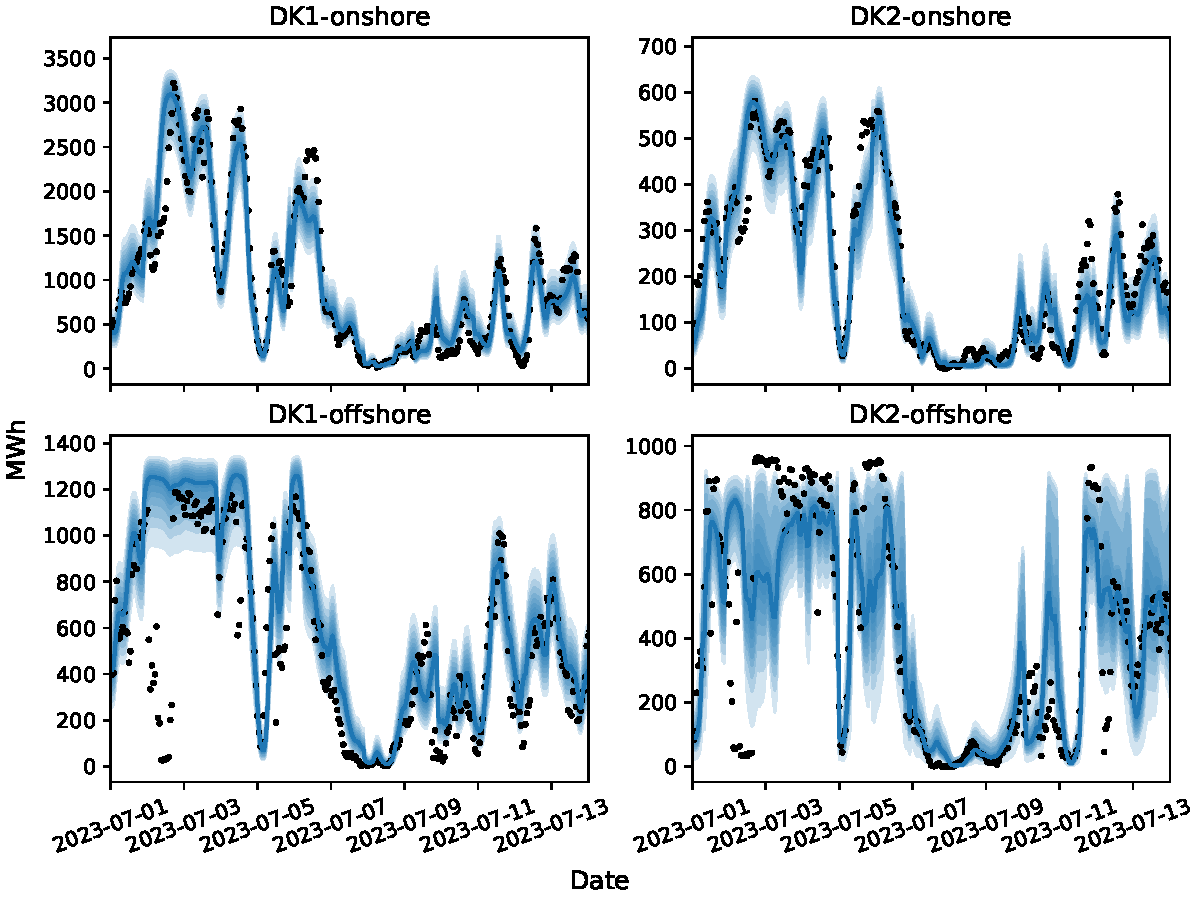
\includegraphics[width=1\linewidth]{Results/Graphs/corrolation_example.pdf}
    \caption{Caption}
    \label{fig:forecastexample}
\end{figure}

\begin{tabular}{llrrrrr}
\toprule
 &  & Ensembles & Latent & Latent - Marginal & Simple & Simple - Marginal \\
\midrule
\multirow[c]{5}{*}{DK1-offshore} & MAE & 138.74 & 118.90 & 119.00 & 116.75 & 116.64 \\
\cline{2-7}
 & RMSE & 193.46 & 176.06 & 176.20 & 171.69 & 171.69 \\
\cline{2-7}
 & CRPS & 107.67 & 87.09 & 86.80 & 86.52 & 86.69 \\
\cline{2-7}
 & VarS & 29.65 & 26.36 & 31.90 & 26.50 & 33.44 \\
\cline{2-7}
 & Geometric Mean Score & 96.21 & 83.26 & 87.29 & 82.33 & 87.29 \\
\cline{1-7} \cline{2-7}
\multirow[c]{5}{*}{DK1-onshore} & MAE & 192.07 & 181.74 & 181.89 & 201.67 & 201.67 \\
\cline{2-7}
 & RMSE & 263.32 & 258.65 & 259.08 & 282.17 & 282.17 \\
\cline{2-7}
 & CRPS & 138.56 & 131.14 & 132.11 & 149.22 & 148.53 \\
\cline{2-7}
 & VarS & 36.60 & 36.38 & 49.99 & 52.55 & 66.92 \\
\cline{2-7}
 & Geometric Mean Score & 126.55 & 122.38 & 132.82 & 145.34 & 154.22 \\
\cline{1-7} \cline{2-7}
\multirow[c]{5}{*}{DK2-offshore} & MAE & 158.55 & 124.73 & 124.46 & 141.50 & 141.39 \\
\cline{2-7}
 & RMSE & 239.70 & 181.04 & 181.03 & 206.90 & 206.89 \\
\cline{2-7}
 & CRPS & 124.22 & 88.32 & 88.70 & 99.16 & 99.26 \\
\cline{2-7}
 & VarS & 30.68 & 30.49 & 42.55 & 31.94 & 45.57 \\
\cline{2-7}
 & Geometric Mean Score & 109.71 & 88.31 & 96.03 & 98.13 & 107.25 \\
\cline{1-7} \cline{2-7}
\multirow[c]{5}{*}{DK2-onshore} & MAE & 82.52 & 39.85 & 39.86 & 38.26 & 38.23 \\
\cline{2-7}
 & RMSE & 112.76 & 55.90 & 55.96 & 52.92 & 52.88 \\
\cline{2-7}
 & CRPS & 63.68 & 28.68 & 28.76 & 28.36 & 28.63 \\
\cline{2-7}
 & VarS & 10.30 & 8.27 & 10.75 & 8.33 & 12.07 \\
\cline{2-7}
 & Geometric Mean Score & 49.71 & 26.96 & 28.82 & 26.30 & 28.91 \\
\cline{1-7} \cline{2-7}
\bottomrule
\end{tabular}

